\documentclass{article}
\usepackage{wasysym}
\usepackage{textcomp}
\usepackage{tikz}

\newcommand{\crel}{
	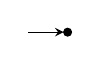
\begin{tikzpicture}[baseline={([yshift=-.8ex]current bounding box.center)}]
		\draw [->, >=stealth] (0,0) -- (0.45,0); 
		\draw [fill] (0.5,0) circle (0.05);
	\end{tikzpicture}
}

\newcommand{\rrel}{
	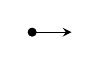
\begin{tikzpicture}[baseline={([yshift=-.8ex]current bounding box.center)}]
		\draw [fill] (0,0) circle (0.05);
		\draw [->, >=stealth] (0.05,0) -- (0.5,0);
	\end{tikzpicture}
}

\newcommand{\mrel}{
	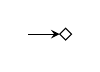
\begin{tikzpicture}[baseline={([yshift=-.8ex]current bounding box.center)}]
		\draw [->, >=stealth] (0,0) -- (0.4,0);
		\draw (0.4,0) -- (0.475,0.075) -- (0.55,0) -- (0.475,-0.075) -- cycle;
	\end{tikzpicture}
}

\newcommand{\irel}{
	\begin{tikzpicture}[baseline={([yshift=-.8ex]current bounding box.center)}]
		\draw [->, >=stealth] (0,0) -- (0.4,0);
		\draw (0.41,0) -- (0.55,0);
		\draw (0.48,-0.07) -- (0.48, 0.07); 
	\end{tikzpicture}
}

\newcommand{\erel}{
	\begin{tikzpicture}[baseline={([yshift=-.8ex]current bounding box.center)}]
		\draw [->, >=stealth] (0,0) -- (0.4,0);
		\draw (0.41,0) -- (0.55,0);
		\draw (0.48, 0.05) circle (0.02);
		\draw (0.48, -0.05) circle (0.02); 
	\end{tikzpicture}
}

\begin{document}
	\noindent
	Workflow: $G=(V,E)$ \\
	Activities: $V=\{v_1,\ \dots, v_n\}$ \\ %missing event states
	Activity States: $S=\{s_1,\ \dots, s_n\}$, where $s_i \subseteq \{Executed, Pending, Included\}$\\
	Relation ($E$): $R=($condition, response, milestone, include, exclude$)$, $e=(v_x, v_y, r_i)$, $E=\{e_1,\ \dots, e_m\}$\\
	Actors: $P =\{$Alice ($A$), Bob ($B$)$\}$.\\
	History, $H_A(t)$, $H_B(t)$: Sequence of activity executions up to, and at time $t$, as perceived by $A$ and $B$, respectively.\\
	Execution: $(v_i, t, p_i)$, where $v_i$ is the activity executed at time $t$, executed by actor $p_i$.\\
	%History, $H(t)$: State of the entire workflow at time $t$

	What we want to achieve:
	\begin{description}
		%\item[Concurrency]: If $H_A(t_1) = H_B(t_1)$
		\item[Correctness]: Any DCR graph must 
		\item  
	\end{description}
	$H_A(t) \subset H_A(t+1)$
	No execution violates DCR rules

\end{document}